\chapter{Wykład 14. Zarządzanie ryzykiem w projekcie informatycznym}

\section{Macierz ryzyka}
% strona 27

Ten wirtualny warsztat jest beznadziejny.

% ===========================================================================

\section{Rejestr ryzyka projektowego}
% strona 36

Ten wirtualny warsztat jest beznadziejny.

% ===========================================================================

\section{Analiza jakościowa i ilościowa SWOT}
% strona 48

\begin{figure}[h]
\begin{center}
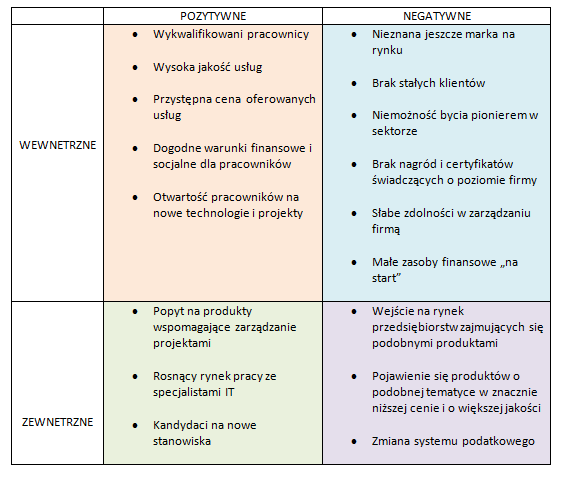
\includegraphics[scale=1]{swot.png}
\caption[Analiza SWOT]{Analiza SWOT}
\label{rysunekProces}
\end{center}
\end{figure}

% ===========================================================================

\section{Analiza jakościowa ryzyka}
% strona 54

Ten wirtualny warsztat jest beznadziejny.

% ===========================================================================

\section{Analiza ilościowa ryzyka}
% strona 62

Ten wirtualny warsztat jest beznadziejny.

% ===========================================================================

\section{Plany reakcji na ryzyko}
% strona 75

\begin{figure}[h]
\begin{center}
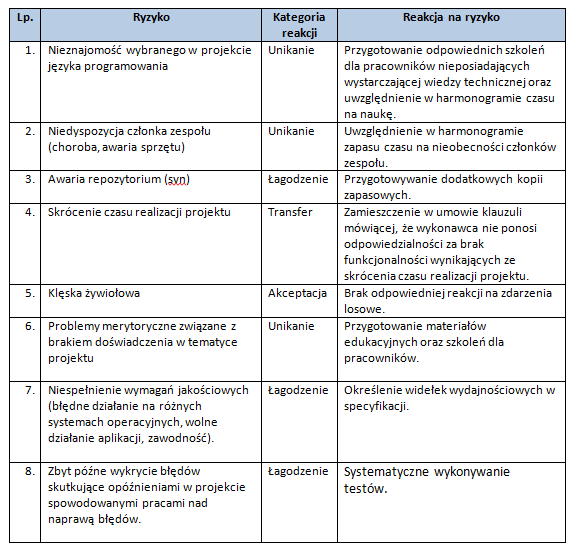
\includegraphics[scale=1]{planreakcji.png}
\caption[Plan reakcji na ryzyko]{Plan reakcji na ryzyko}
\label{rysunekProces}
\end{center}
\end{figure}


